\documentclass[11pt,a4paper]{article}

\usepackage[utf8]{inputenc}
\usepackage{amsmath}
\usepackage{amsfonts}
\usepackage{amssymb}
\usepackage{parskip} 
\usepackage[left=1.5cm,right=1.5cm,top= 1.5cm,bottom=1.5cm]{geometry}
\usepackage{graphicx}
\usepackage{float}
\usepackage{subcaption} 
\usepackage{multicol}

\usepackage{Sweave}
\begin{document}
\Sconcordance{concordance:SemiMarkov_Paper.tex:SemiMarkov_Paper.Rnw:%
1 13 1 1 0 4 1 1 6 1 1 1 12 38 1 1 2 11 0 1 2 4 1 1 4 7 0 1 2 9 1 1 33 %
6 1 1 8 5 0 1 2 19 0 1 2 3 1 1 5 5 0 1 2 17 0 1 3 2 1 1 5 5 0 1 2 35 0 %
1 2 8 1 1 7 2 1 1 5 5 0 1 1 15 0 1 3 49 0 1 4 53 0 1 2 2 1 1 4 1 2 3 1 %
1 5 10 0 1 2 6 1 1 5 5 0 1 1 15 0 1 3 49 0 1 4 53 0 1 2 2 1 1 5 1 2 3 1 %
1 6 10 0 1 2 6 1 1 5 5 0 1 1 15 0 1 3 49 0 1 4 53 0 1 2 2 1 1 5 1 2 3 1 %
1 6 10 0 1 2 6 1 1 5 5 0 1 1 15 0 1 3 49 0 1 4 53 0 1 2 2 1 1 5 1 2 3 1 %
1 6 10 0 1 2 10 1 1 5 5 0 1 1 51 0 1 3 42 0 1 3 53 0 1 2 30 1}

  	

%create global options for evaluating all R codes in my document

% load required packages

\newpage

\begin{abstract}
\noindent\textbf{Abstract}—The purpose of this study is to model the transitions of HIV viral load of patients under differentiated care using homogeneous semi-Markov processes. The model focuses on the patient’s WHO staging and DCM as factors. A sample of 366 patients ordered chronologically  was taken from a hospital record in Kenya.  A total of 918 states were observed where 39.87\% and 60.13\% are in similar and different states respectively. The states of viral load were defined based on the WHO HIV staging classification of HIV/AIDS infected patients, we picked 3 states viral loads as follows: <400(stage 1); 400 to 600 (stage 2); 600 to 999 (stage 3). The three states are living states. We assume the living states communicate with each other. We don’t have the absorbing states.\\

\textbf{Keywords:} disease transition, homogeneous semi-Markov process, HIV/AIDS

\end{abstract}


\section{Introduction}
For more than four decades now, human immunodeficiency virus (HIV) infection has become the epicentre of the diseases challenging humanity and a major focus of public health specialists and researchers. Laboratory measurement of plasma HIV viral load is used to determine the extent of body immune destruction as well as monitor the disease progression. The World Health Organization (WHO) has put in place clinical staging that uses various clinical parametres to aid in managing the HIV patients. The WHO staging puts both adults and children into 4 hierarchical stages ;stage 1(asymptomatic) to stage 4 (AIDS) depending on viral load suppression and various observable clinical conditions.\\

The purpose of this study is
\begin{enumerate}
    \item[(a.)] What is the effects of putting patients under differentiated care(DCM) on their viral load?
    \item[(b.)] To model the transition states of HIV viral load of patients under DCM
    \item[(b.)] To determine and select the appropriate distributions which describes the various transition states.

\end{enumerate}


\section{Literature Overview}
\begin{multicols}{2}
In most longitudinal medical studies on the progression of healthy individuals to chronic diseases, the natural development is often expressed in terms of distinct states. The analyses in such studies where individuals may transition among several states are performed by using multi-state models which can either be discrete or continuous. Multi-state models based on the discrete-time Markov chain have become popular in analyzing longitudinal data collected in chronic disease studies. Such models are also called Markov chain transitional models (Agresti 2002). Kryscio, Schmitt, and Salazar (2006) used a Markov chain model to identify risk factors
associated with transitions from cognitively normal to various forms of mild cognitive impairment (MCI) and then from MCI into early dementia, with death before dementia as a competing state. A continuous-time MSM is a model for a continuous time stochastic process allowing individuals to move among a finite number of states (Meira-Machado et al. (2009). There exists an extensive literature on continuous-time MSMs (see, e.g., Hougard (1999) or Commenges (1999))., Hubbard and Zhou (2011), or Joly, Commenges, and Letenneur (1998), Joly, and Commenges (1999), Joly et al. (2002). Applications of continuous-time MSMs can be found in liver cirrhosis (Andersen, Esbjerg, and Sorensen (2000)), dementia (Joly, Commenges, and Letenneur 1998, Joly, and Commenges 1999, Joly et al. 2002; Hubbard and Zhou 2011) among others.
The use of multi-state Markov models to analyze the factors associated with transitions between different states of chronicity has been suggested for chronic diseases and the cost-effectiveness of various therapeutic regimes (Shih et al., 2007; Pan et al., 2007; Gil et al., 2007). Recent studies have shown that the predicted probability of patients that changing their status given
his/her current status allows the measurements of medical scientific progresses due to the advances in the treatment of the HIV/AIDS (D'Amico et al., 2009). Masala et al. (2014; Goshu and Dessie, 2013; Giuseppe et al., 2007) analyzed HIV/AIDS dynamic evolution as defined by CD4 levels from a macroscopic point of view by means of homogeneous semi-Markov stochastic processes Numerical analyses of the homogeneous semi-Markov process are dealt by
Corradi et al. (2004; Janssen and Manca, 2001). Other more readings include (Davidov and Zelen, 2000; Viladent and Van Ackere, 2007; Satten and Sternberg, 1999; Baryarama et al., 2005). In this study, the author, a procedure to obtain the parameters in a model with covariates has been reported (Maciulis et al., 2009; Gentlemann et al.,1985; Mathieu et al., 2007; P<U+0450>rez-Oc<U+03CC>n et al., 2001).
\end{multicols}

\section{Data Exploration and Analysis}
  \subsection{Data Description}
WHO staging (0 for any staging greater than 1 i.e. 2,3 and 4. and 1 for stage 1), DCM(yes= 1, No= 0), AgeGroup(adult= 1, child= 0) and Sex(Female= 1, Male= 0)  \\
A total of 552 different transitions states and 366 HIV patients was studied as shown in the table below.


\begin{minipage}{0.45\textwidth}
\begin{Schunk}
\begin{Soutput}
$table.state
    1   2   3
1 151  94  43
2 112 115  70
3 114 119 100

$Ncens
[1] 366
\end{Soutput}
\end{Schunk}
\end{minipage}%
\hfill
\begin{minipage}{0.45\textwidth}
\begin{tabular}{|p{\textwidth}}
Transition probability matrix
\begin{Schunk}
\begin{Soutput}
            1         2         3
  1 0.5243056 0.3263889 0.1493056
  2 0.3771044 0.3872054 0.2356902
  3 0.3423423 0.3573574 0.3003003
\end{Soutput}
\end{Schunk}
\end{tabular}
\end{minipage}%
\\

The probability of transitioning from a lower state to a higher state is lower than the vice versa. There is a high probability of patient remaining in the same state, more illustrated by 1-->1 transition.\\

Drawing of HIV transition states\\
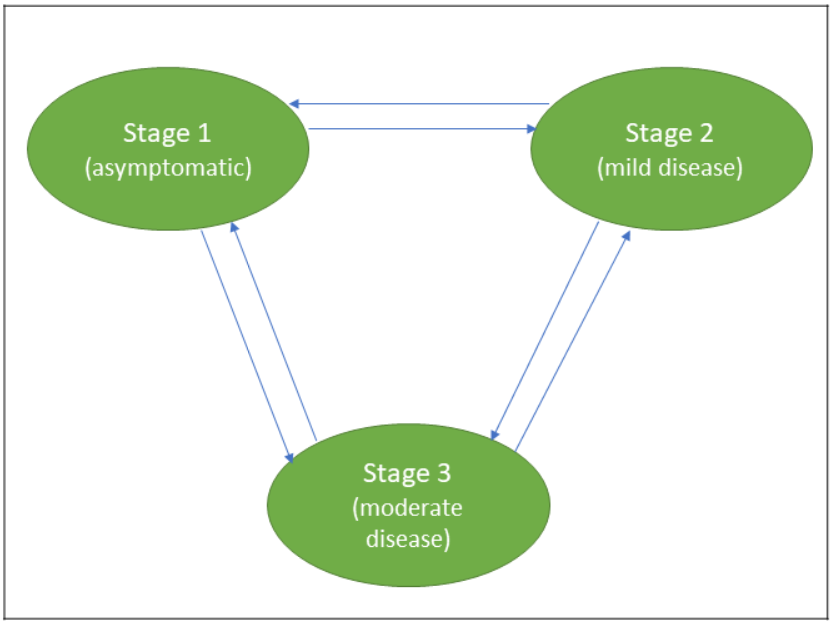
\includegraphics[scale=0.2]{diagram2.PNG}




\subsection{Model Fitting and Selection}
  
\textbf{Weibull distribution}\\

The transitions between the different states are significant since all the p-values < 10\%, at \(\alpha\) = 10\%.
\begin{Schunk}
\begin{Soutput}
Iter: 1 fn: 1615.2486	 Pars:  9.36243 2.94492 6.63966 3.06917 2.43166 5.72270 1.35845 3.90000 1.41184 3.58816 7.68670 1.61996 0.83719 0.73928 0.34749
Iter: 2 fn: 1615.2486	 Pars:  9.36258 2.94492 6.63965 3.06917 2.43166 5.72268 1.35843 3.90001 1.41184 3.58815 7.68668 1.61996 0.83719 0.73928 0.34749
solnp--> Completed in 2 iterations
\end{Soutput}
\begin{Soutput}
$Sigma
  Type Index Transition Sigma   SD Lower_CI Upper_CI Wald_H0 Wald_test p_value
1 dist     1     1 -> 2 9.363 0.84     7.72    11.01    1.00     99.16 <0.0001
2 dist     2     1 -> 3 2.945 0.13     2.70     3.19    1.00    236.13 <0.0001
3 dist     3     2 -> 1  6.64 0.47     5.72     7.56    1.00    143.66 <0.0001
4 dist     4     2 -> 3 3.069 0.11     2.85     3.29    1.00    335.01 <0.0001
5 dist     5     3 -> 1 2.432 0.03     2.37     2.49    1.00   2049.64 <0.0001
6 dist     6     3 -> 2 5.723 0.34     5.06     6.38    1.00    197.66 <0.0001

$Nu
  Type Index Transition    Nu   SD Lower_CI Upper_CI Wald_H0 Wald_test p_value
1 dist     7     1 -> 2 1.358 0.12     1.12     1.59    1.00      8.91  0.0028
2 dist     8     1 -> 3   3.9 0.41     3.09     4.71    1.00     49.17 <0.0001
3 dist     9     2 -> 1 1.412 0.11     1.20     1.63    1.00     14.09  0.0002
4 dist    10     2 -> 3 3.588 0.29     3.02     4.16    1.00     79.49 <0.0001
5 dist    11     3 -> 1 7.687 0.44     6.83     8.55    1.00    233.01 <0.0001
6 dist    12     3 -> 2  1.62 0.12     1.38     1.86    1.00     26.33 <0.0001
\end{Soutput}
\end{Schunk}

\textbf{Exponential distribution}

The p-value for transition between 1-->3 is \textbf{0.1726} which is greater than  =10\%.This transition under exponential is insignificant. 
\begin{Schunk}
\begin{Soutput}
Iter: 1 fn: 1894.9202	 Pars:  9.66638 6.90269 5.00360 7.24220 3.99801 5.19016 0.73265 0.56477 0.45916
Iter: 2 fn: 1894.9202	 Pars:  9.66675 6.90192 5.00366 7.24206 3.99801 5.19017 0.73267 0.56478 0.45916
solnp--> Completed in 2 iterations
\end{Soutput}
\begin{Soutput}
$Sigma
  Type Index Transition Estimation   SD Lower_CI Upper_CI Wald_H0 Wald_test
1 dist     1     1 -> 2      9.667 2.16     5.43    13.91    1.00     16.04
2 dist     2     1 -> 3      6.902 4.33    -1.58    15.38    1.00      1.86
3 dist     3     2 -> 1      5.004 1.09     2.88     7.13    1.00     13.60
4 dist     4     2 -> 3      7.242 1.79     3.74    10.74    1.00     12.20
5 dist     5     3 -> 1      3.998 0.66     2.70     5.29    1.00     20.57
6 dist     6     3 -> 2       5.19 0.71     3.81     6.57    1.00     35.21
  p_value
1  0.0001
2  0.1726
3  0.0002
4  0.0005
5 <0.0001
6 <0.0001
\end{Soutput}
\end{Schunk}

\textbf{Exponentiated weibull distribution}
The p-value for transition between 1-->3 is \textbf{0.729} which is greater than  10\%.This transition under exponential-weibul is insignificant.\\
